\documentclass[a4paper,10pt]{article}
\usepackage{listings}
\usepackage{color}
\usepackage{algorithm2e}
\usepackage{graphicx}
\usepackage{epstopdf}
\usepackage{multirow}
\usepackage[margin=1.0in]{geometry}
\usepackage{amsmath,amsthm,amssymb}
 
\definecolor{dkgreen}{rgb}{0,0.6,0}
\definecolor{gray}{rgb}{0.5,0.5,0.5}
\definecolor{mauve}{rgb}{0.58,0,0.82}
 
\lstset{ %
  language=C++,                % the language of the code
  basicstyle=\footnotesize,           % the size of the fonts that are used for the code
  numbers=left,                   % where to put the line-numbers
  numberstyle=\tiny\color{gray},  % the style that is used for the line-numbers
  stepnumber=1,                   % the step between two line-numbers. If it's 1, each line 
                                  % will be numbered
  numbersep=5pt,                  % how far the line-numbers are from the code
  backgroundcolor=\color{white},      % choose the background color. You must add \usepackage{color}
  showspaces=false,               % show spaces adding particular underscores
  showstringspaces=false,         % underline spaces within strings
  showtabs=false,                 % show tabs within strings adding particular underscores
  frame=single,                   % adds a frame around the code
  rulecolor=\color{black},        % if not set, the frame-color may be changed on line-breaks within not-black text (e.g. commens (green here))
  tabsize=2,                      % sets default tabsize to 2 spaces
  captionpos=b,                   % sets the caption-position to bottom
  breaklines=true,                % sets automatic line breaking
  breakatwhitespace=false,        % sets if automatic breaks should only happen at whitespace
  title=\lstname,                   % show the filename of files included with \lstinputlisting;
                                  % also try caption instead of title
  keywordstyle=\color{blue},          % keyword style
  commentstyle=\color{dkgreen},       % comment style
  stringstyle=\color{mauve},         % string literal style
  escapeinside={\%*}{*)},            % if you want to add LaTeX within your code
  morekeywords={*,...}               % if you want to add more keywords to the set
}

% Title Page
\title{Assignment 2: Dynamic Programming project}
\author{Francis Vo, Soo-Hyun Yoo}

\setlength{\parindent}{1cm}
\setlength{\parskip}{1em}

\begin{document}
	\maketitle

	\section{Problem 1: mmmm ... pork}
	\subsection{Mathematical}
\subsubsection{Objective function} 
%max\\
%$8 * ham\_f + 12 * ham\_r + 11 * ham\_o + $\\
%$4 * bellies\_f + 12 * bellies\_r + 7 * bellies\_o + $\\
%$4 * picnics\_f + 13 * picnics\_r + 9 * picnics\_o$
\begin{tabular}{ccccccc}
&$8 * ham\_f $& $+$& $ 12 * ham\_r$& $ + $& $11 * ham\_o$& $+ $\\
max &$4 * bellies\_f $& $+ $& $12 * bellies\_r$& $ + $& $7 * bellies\_o$& $ +$\\
&$4 * picnics\_f $& $+ $& $13 * picnics\_r $& $+$& $ 9 * picnics\_o$
\end{tabular}


\subsubsection{Constraints} 
\begin{tabular}{rcl}
 $ham\_f + ham\_r + ham\_o$& $\le$ &$480$\\
$bellies\_f + bellies\_r + bellies\_o$ &$ \le$ &$ 400$\\
$picnics\_f + picnics\_r + picnics\_o$ &$ \le$ &$ 230$\\
$ham\_r + bellies\_r + picnics\_r$ &$\le $ &$420$\\
$ham\_o + bellies\_o + picnics\_o $ &$\le$ &$ 250$\\
\end{tabular}

	\subsection{Standard}
\subsubsection{Objective function} 
\begin{tabular}{ccccccc}
&$8 * ham\_f $& $+$& $ 12 * ham\_r$& $ + $& $11 * ham\_o$& $+ $\\
max &$4 * bellies\_f $& $+ $& $12 * bellies\_r$& $ + $& $7 * bellies\_o$& $ +$\\
&$4 * picnics\_f $& $+ $& $13 * picnics\_r $& $+$& $ 9 * picnics\_o$
\end{tabular}


\subsubsection{Constraints} 
%$ham\_f + ham\_r + ham\_o + ham\_remain = 480$\\
%$bellies\_f + bellies\_r + bellies\_o + bellies\_remain = 400$\\
%$picnics\_f + picnics\_r + picnics\_o + picnics\_remain = 230$\\
%$ham\_r + bellies\_r + picnics\_r + smoke\_reg = 420$\\
%$ham\_o + bellies\_o + picnics\_o + smoke\_over = 250$\\
%$ham\_remain, bellies\_remain, picnics\_remain, smoke\_reg, smoke\_over \ge 0$\\

% Francis's try at making it look nice
\begin{tabular}{rcl}
 $ham\_f + ham\_r + ham\_o + ham\_remain$& $=$ &$480$\\
$bellies\_f + bellies\_r + bellies\_o + bellies\_remain$ &$ =$ &$ 400$\\
$picnics\_f + picnics\_r + picnics\_o + picnics\_remain$ &$ =$ &$ 230$\\
$ham\_r + bellies\_r + picnics\_r + smoke\_reg $ &$= $ &$420$\\
$ham\_o + bellies\_o + picnics\_o + smoke\_over $ &$=$ &$ 250$\\
$ham\_remain, bellies\_remain, picnics\_remain, smoke\_reg, smoke\_over$ &$ \ge$ &$ 0$\\
\end{tabular}


	\subsection{Matrix}
	Max($f'*x$)
	
	\[ f' = \left( \begin{array}{ccccccccc}
	8 & 14 & 11 & 
	4 & 12 & 7 & 
	4 & 13 & 9  
	\end{array} \right)\]
	

	\[ a = \left( \begin{array}{ccccccccc}
	1 & 1 & 1 & 0 & 0 & 0 & 0 & 0 & 0 \\
	0 & 0 & 0 & 1 & 1 & 1 & 0 & 0 & 0 \\
	0 & 0 & 0 & 0 & 0 & 0 & 1 & 1 & 1 \\
	0 & 1 & 0 & 0 & 1 & 0 & 0 & 1 & 0 \\
	0 & 0 & 1 & 0 & 0 & 1 & 0 & 0 & 1 \\
	\end{array} \right)\]
	
	\[ b = \left( \begin{array}{c}
	480\\
	400\\
	230\\
	420\\
	250
	\end{array} \right)\]
	

	\[ x = \left( \begin{array}{c}
	ham\_f\\
	ham\_r\\
	ham\_o\\
	bellies\_f\\
	bellies\_r\\
	bellies\_o\\
	picnics\_f\\
	picnics\_r\\
	picnics\_o
	\end{array} \right)\]

	\subsection{Code}
	      \lstinputlisting{pork.mod}

	\newpage
	\subsection{Solution}
	Total net profit: \$10,910\\
	\begin{tabular}{lccc}
\hline
	& fresh & smoked on regular time & smoked on overtime\\
\hline
	hams & 440 & 0 & 40\\
	bellies & 0 & 400 & 0\\
	picnics & 0 & 20 & 210
	\end{tabular}
	%\lstinputlisting{pork.sol}

	\subsection{GNU Linear Programming Kit}
	      We used a glpsol inputing a model file, pork.mod, and then it outputs a solution file, pork.sol.  The command we used is ``glpsol -m pork.mod -o pork.sol''



	\section{Problem 2: least squares isn’t good enough for me}
		
	\subsection{Mathematical}
	\subsubsection{Objective function} 
	min t

	\subsubsection{Constraints}
	for each point

	\begin{tabular}{rcl}
		$|point.x - b|$&$ <= $&$t$\\
		$|a*(point.x)+b*(point.y)-c|$&$ <= $&$t$
	\end{tabular}


	\subsection{Standard}
	\subsubsection{Objective function} 
	min t

	\subsubsection{Constraints}
	for each point

	\begin{tabular}{rcl}
		$point.x - b + point.v$&$ = $&$t$\\
		$point.x - b$&$ \ge $&$-t$\\
		$a*(point.x)+b*(point.y)-c + point.z$&$ = $&$t$\\
		$a*(point.x)+b*(point.y)-c $&$\ge$&$ -t$\\
		$point.v, point.z $&$\ge$&$ 0$
	\end{tabular}

 

	\subsection{Code}
	\lstinputlisting{bestFit.mod}

	\subsection{Solution}
	$a=-8.8$\\
	$b=5.5$\\
	$c=12$

	%\lstinputlisting{bestFit2.sol}

	\subsection{Plot}
		\begin{figure}[!htb]
			\centering
			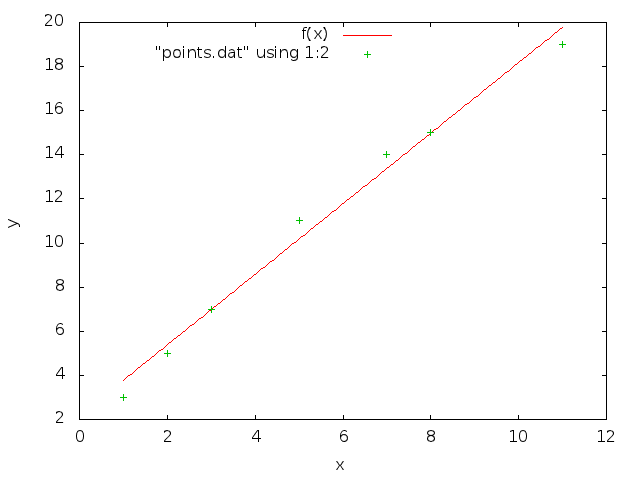
\includegraphics[scale=.5]{plot.png}
			\caption{points and best fit line}
			\label{fig:algcomp}
		\end{figure}

\end{document}
